%=====================================================================
%  Coursework - Code Tour
%  Compile:  tectonic -X compile code-tour.tex --outdir build
%         or ./build-tour.sh
%=====================================================================
\documentclass[11pt,letterpaper]{article}

\usepackage[T1]{fontenc}
\usepackage[utf8]{inputenc}
\usepackage{lmodern}
\usepackage[letterpaper,margin=1in,headheight=14pt]{geometry}
\usepackage{microtype}
\usepackage{graphicx}
\usepackage{xcolor}
\usepackage{enumitem}
\usepackage{booktabs}
\usepackage{array}
\usepackage{titlesec}
\usepackage{fancyhdr}
\usepackage{listings}
\usepackage[most,breakable]{tcolorbox}
\usepackage{caption}
\usepackage[hidelinks,colorlinks=true,linkcolor=linknavy,urlcolor=linknavy]{hyperref}

\definecolor{linknavy}{HTML}{1F4E79}
\definecolor{inkdark}{HTML}{1A1A1A}
\definecolor{rulegrey}{HTML}{BFBFBF}
\definecolor{qblue}{HTML}{1F4E79}
\definecolor{keygreen}{HTML}{2E6B4F}
\definecolor{keygreenbg}{HTML}{EDF5F0}
\definecolor{codebg}{HTML}{F6F6F4}
\definecolor{muted}{HTML}{6B625A}

\pagestyle{fancy}
\fancyhf{}
\renewcommand{\headrulewidth}{0.4pt}
\fancyhead[L]{\small Coursework \textendash\ code tour}
\fancyhead[R]{\small\thepage}

\titleformat{\section}{\normalfont\Large\bfseries\color{inkdark}}{\thesection}{0.8em}{}
\titleformat{\subsection}{\normalfont\large\bfseries\color{inkdark}}{\thesubsection}{0.8em}{}
\titleformat{\subsubsection}{\normalfont\normalsize\bfseries\color{inkdark}}{}{0em}{}

\lstdefinestyle{ct}{
  basicstyle=\ttfamily\footnotesize,
  backgroundcolor=\color{codebg},
  frame=single, rulecolor=\color{rulegrey},
  breaklines=true, columns=fullflexible, keepspaces=true,
  showstringspaces=false, xleftmargin=6pt, framexleftmargin=6pt,
  aboveskip=8pt, belowskip=8pt,
  keywordstyle=\color{qblue}\bfseries,
  commentstyle=\color{keygreen}\itshape,
}
\lstset{style=ct}
\lstdefinelanguage{none}{keywords={}, sensitive=false}

\newtcolorbox{keypoint}[1][]{
  breakable, enhanced, colback=keygreenbg, colframe=keygreen,
  boxrule=0pt, leftrule=3pt, arc=1pt, left=8pt, right=8pt, top=6pt, bottom=6pt,
  fonttitle=\bfseries\small, title={#1}, coltitle=keygreen,
  attach boxed title to top left={xshift=6pt,yshift=-2pt},
  boxed title style={colback=keygreenbg, boxrule=0pt, sharp corners}}

\newcommand{\code}[1]{\texttt{\small #1}}
\newcommand{\term}[1]{\textbf{#1}}
\captionsetup{font=small, labelfont={bf,color=qblue}}
\setlist[itemize]{itemsep=2pt, topsep=4pt, leftmargin=1.3em}
\setlength{\parskip}{0.45em}
\setlength{\parindent}{0pt}
\raggedbottom

\begin{document}

\begin{center}
  {\Huge\bfseries Coursework}\\[4pt]
  {\Large\mdseries Code tour}\\[10pt]
  {\color{muted} A file-by-file walk through the repository:\\
   what each thing is, why it exists, and what to read first.}\\[8pt]
  {\small\color{muted}\href{https://github.com/jawaadjariwala/coursework-takeoff}{github.com/jawaadjariwala/coursework-takeoff}}
\end{center}

\vspace{6pt}
\hrule
\vspace{14pt}

\begin{keypoint}[If you have fifteen minutes]
Read \code{src/coursework/geometry/junctions.py}, then \code{tests/oracle.py},
then run \code{coursework ui -{}-demo-plan}. Everything else in the repository
is scaffolding around those two ideas.
\end{keypoint}

\tableofcontents
\vspace{10pt}

\section{What the project is}

A desktop tool that reads masonry quantities off a building plan. You trace
the walls, say what each one is made of, and it tells you how many blocks,
how many bricks, how many bags of mortar.

The part that makes it more than a calculator is what happens where two
walls meet. Masonry is measured along wall centerlines, and that convention
is exactly self-correcting at an L corner and self-correcting nowhere else.
The solver classifies every junction and corrects each one, and the report
shows both numbers: what the raw centerline total claims, and what it
actually is.

\begin{figure}[h]
\centering
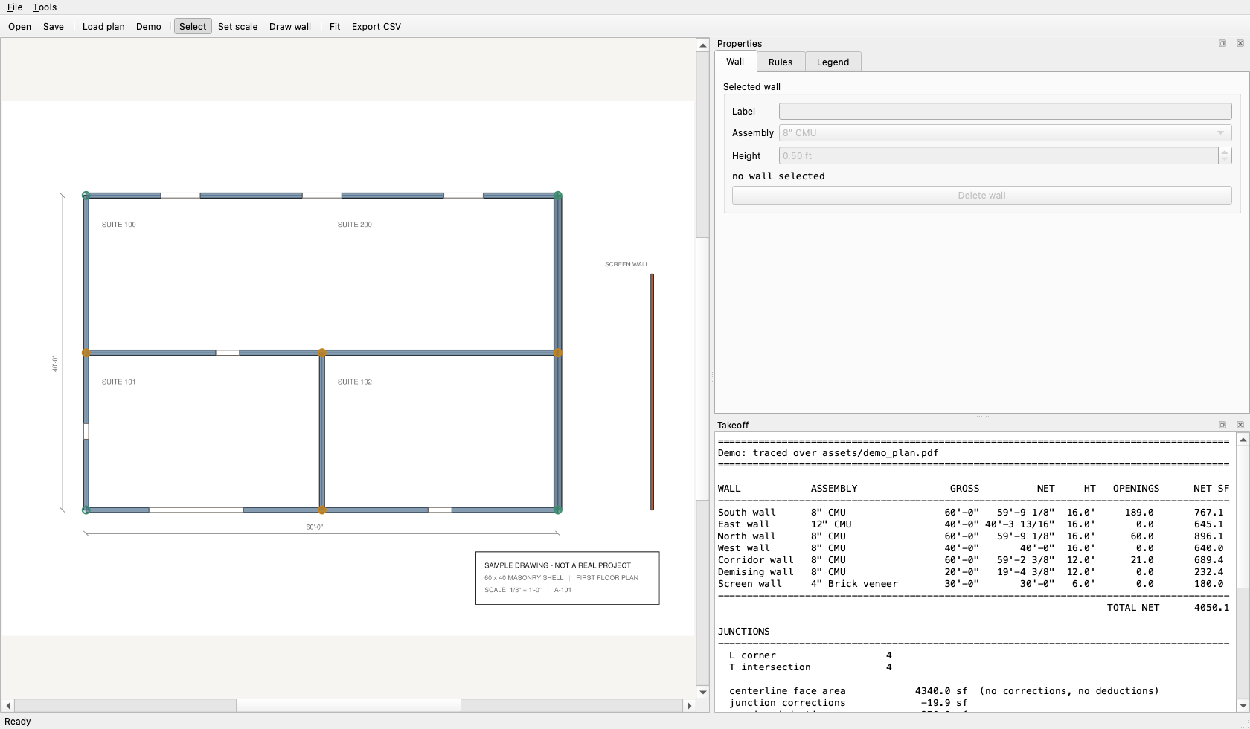
\includegraphics[width=\textwidth]{img/app_plan.png}
\caption{The application with the demo building traced over the sample
drawing. The traced walls sit exactly on the drawn walls and the openings
land exactly in the drawn gaps, which is a visual proof that the scale
calibration is correct. Coloured dots mark junctions: green where the
centerline self-corrects, amber where material moved.}
\end{figure}

\section{Running it}

\begin{lstlisting}[language=none]
python -m venv .venv && source .venv/bin/activate
pip install -e ".[dev]"

coursework ui --demo-plan     # the app, traced over the sample drawing
coursework ui                 # the app, no underlay
coursework report --demo      # the takeoff as text
coursework export --demo -o takeoff.csv
coursework save-demo job.ctk  # write the demo to a project file
coursework bench              # junction detection benchmark
pytest -q                     # 177 tests
ruff check src tests tools    # lint
\end{lstlisting}

\section{The map}

\begin{lstlisting}[language=none]
src/coursework/
  model/        plain data. No Qt, no geometry library, no database.
  geometry/     the junction solver. Pure Python and NumPy.
  quantities/   materials, arithmetic, report rendering.
  store/        SQLite project file with migrations.
  ui/           PySide6. The only package allowed to import Qt.
  demo.py       the sample building
  cli.py        command line entry point
  bench.py      performance benchmark
tools/          sample plan generator (dev only, not shipped)
tests/          177 tests including the independent oracle
docs/           decisions, this tour, images
assets/         the sample floor plan PDF
.github/        CI
\end{lstlisting}

The layering rule is \textbf{nothing outside \code{ui/} imports Qt}, and it
is enforced by a test, not by discipline. That is what lets the engine run
headless: testable in CI with no display, benchmarkable in a loop, drivable
from a command line.

\section{\texttt{model/} \textendash\ the data}

No behaviour beyond validation. Everything else operates on these objects.

\subsection{\texttt{types.py} (168 lines)}

\begin{itemize}
  \item \term{Assembly} \textendash\ one masonry material at one nominal
    thickness. Carries \code{thickness\_in}, \code{units\_per\_sf},
    \code{mortar\_bags\_per\_100\_units}, and a \code{priority} that breaks
    ownership ties at junctions. Structural block outranks veneer because
    the block runs continuous through a junction and the veneer stops
    against it.
  \item \term{Wall} \textendash\ a centerline polyline, an assembly key, a
    height. Rejects fewer than two vertices or a non-positive height at
    construction.
  \item \term{Opening} \textendash\ a rectangular hole on one wall. Stored
    as a \emph{station} (distance along the centerline) rather than an
    absolute point, so it travels with the wall when the wall is edited.
  \item \term{TakeoffSettings} \textendash\ the estimating rules the user is
    allowed to disagree with: waste factor, opening deduction threshold,
    sand per bag.
  \item \term{Project} \textendash\ everything that gets saved.
\end{itemize}

\begin{keypoint}[One unit internally]
Decimal feet everywhere. Thickness is quoted in inches because that is the
trade convention, and converted once. One internal unit removes a whole
class of bug that estimating tools are famous for.
\end{keypoint}

\subsection{\texttt{units.py} (112 lines)}

Feet-and-inches parsing and formatting, the only place that boundary exists.
\code{parse\_ft\_in} accepts what an estimator would actually type:
\code{20'-6"}, \code{20' 6 1/2"}, \code{20-6}, \code{20.5}, \code{6"},
\code{20ft 6in}, and curly quotes. A bare number is read as feet, because
that is what someone typing a wall length means.

\section{\texttt{geometry/} \textendash\ the heart}

\subsection{\texttt{primitives.py} (105 lines)}

Dot, cross, distance, point-to-segment distance, polyline length, and
\code{segment\_intersection}.

\code{segment\_intersection} returns the point \emph{and both parameters}
$t$ and $u$. Those parameters are what the classifier runs on: whether an
intersection lands at a wall's end or in its body is the difference between
an L corner and a T intersection.

Collinear overlap deliberately returns \code{None}. Two walls lying on top
of each other is a tracing error, not a junction, and the solver reports it
rather than inventing a correction.

\code{TOL = 0.02} feet, just under a quarter inch: finer than anyone can
trace on a scanned plan, coarse enough to absorb float noise from the
pixel-to-feet conversion.

\subsection{\texttt{junctions.py} (495 lines) \textendash\ read this one}

The largest and most important file. Its module docstring contains the
derivation.

Wall A along $+x$ with thickness $t_a$, wall B along $+y$ with thickness
$t_b$, both ending at the origin:

\begin{lstlisting}[language=none]
overlap   x in [0,  tb/2],  y in [0,  ta/2]   area = ta*tb/4  counted twice
notch     x in [-tb/2, 0],  y in [-ta/2, 0]   area = ta*tb/4  counted zero times
\end{lstlisting}

Equal for any pair of thicknesses, so they cancel. That is why centerline
measurement works at corners.

\subsubsection{What the file contains, in order}

\begin{itemize}
  \item \code{ContactType} (END / BODY) and \code{JunctionKind} (L / T / X / MULTI)
  \item \code{Contact}, \code{Junction}, \code{Solution} dataclasses
  \item \code{\_segments} \textendash\ flattens walls into segments carrying
    their station offset
  \item \code{naive\_pairs} \textendash\ every cross-wall segment pair,
    $O(n^2)$, the obvious version
  \item \code{grid\_pairs} \textendash\ a uniform grid hash over bounding boxes
  \item \code{find\_junctions} \textendash\ intersects candidates, classifies
    each contact as END or BODY, detects collinear overlap
  \item \code{\_cluster} \textendash\ groups pairwise hits at the same point
    into one node. \textbf{This is where the time actually goes on a large
    plan}; both a quadratic and a spatially hashed version are kept so the
    benchmark can compare and the tests can assert they agree
  \item \code{\_classify} \textendash\ two ENDs is an L, one END is a T, zero
    is an X, three or more contacts is MULTI
  \item \code{\_pick\_owner} \textendash\ highest assembly priority wins,
    lowest wall id breaks ties so the answer never depends on drawing order
  \item \code{\_apply} \textendash\ the corrections, one branch per kind
  \item \code{solve} \textendash\ the public entry point
\end{itemize}

\subsubsection{The corrections}

\begin{center}
\begin{tabular}{@{}lp{8.2cm}@{}}
\toprule
\textbf{Junction} & \textbf{Correction} \\
\midrule
L, same assembly & none; overlap and notch cancel \\
L, mixed assembly & non-owner loses $t_{owner}/4$, owner gains $t_{other}/4$ \\
T intersection & butting wall loses $t_{host}/2$ \\
X crossing & non-owner loses $t_{owner}$ \\
MULTI & pairwise against the owner, and flagged \code{needs\_review} \\
\bottomrule
\end{tabular}
\end{center}

MULTI is the honest limit. Three or more walls at one point get an
approximation and say so in the report warnings, rather than quietly
returning a number.

\section{\texttt{quantities/} \textendash\ from geometry to a bill}

\subsection{\texttt{catalog.py} (95 lines)}

Four assemblies (6", 8", 12" CMU and 4" brick veneer) and the published
constants behind them, with sources named in the docstring. 1.125 units per
square foot for all three block sizes, because they present the same 8x16
face. 6.75 for modular brick. 3 bags of mortar per 100 block, 7 per 1000
brick, 1 CY sand per 7 bags. 5\% waste by default.

Thicknesses are \textbf{actual, not nominal}: an 8" block is 7-5/8" of
material. Using nominal would overstate every junction correction by about
5\%. The docstring also records that sources disagree on mortar, and why the
Titan America figures are the default, rather than picking one silently.

\subsection{\texttt{takeoff.py} (182 lines)}

The arithmetic chain, deliberately short so every step is reportable:

\begin{lstlisting}[language=none]
centerline length
  - junction corrections        -> net length
  x wall height                 -> gross face area
  - openings over the threshold -> net face area
  x units per sf                -> unit count
  x (1 + waste)                 -> ordered count
  -> mortar bags -> sand
\end{lstlisting}

\code{Report} carries both the corrected number and
\code{total\_naive\_area\_sf}, the number an uncorrected takeoff would have
produced, which is what lets the report show the difference.

\subsection{\texttt{render.py} (183 lines)}

\code{as\_text} for the terminal and the app's report panel, \code{as\_csv}
for Excel. The CSV includes a per-junction table with coordinates, owner and
note, so a reviewer can audit every correction rather than trusting the
total.

\section{\texttt{store/} \textendash\ persistence}

\subsection{\texttt{sqlite\_store.py} (208 lines)}

A takeoff is saved as a single SQLite file with the extension \code{.ctk}.

Tables: \code{meta}, \code{project}, \code{wall}, \code{wall\_vertex},
\code{opening}. Foreign keys with \code{ON DELETE CASCADE} so an opening
cannot outlive its wall. \code{CHECK} constraints on geometry. A
\code{MIGRATIONS} list where each entry runs once, with
\code{schema\_version} recording progress, so a file written by an older
build opens in a newer one.

\begin{keypoint}[The whole save is one transaction]
A constraint violation rolls back and leaves the previous file intact, and
there is a test for exactly that, because it is someone's afternoon of work.
\end{keypoint}

Why not JSON: a takeoff is a document, but it is also a thing people query.
"Every opening over 20 sf", "every wall of 12-inch block" are one line of
SQL and a page of Python over parsed JSON.

\section{\texttt{ui/} \textendash\ the only Qt}

\begin{figure}[h]
\centering
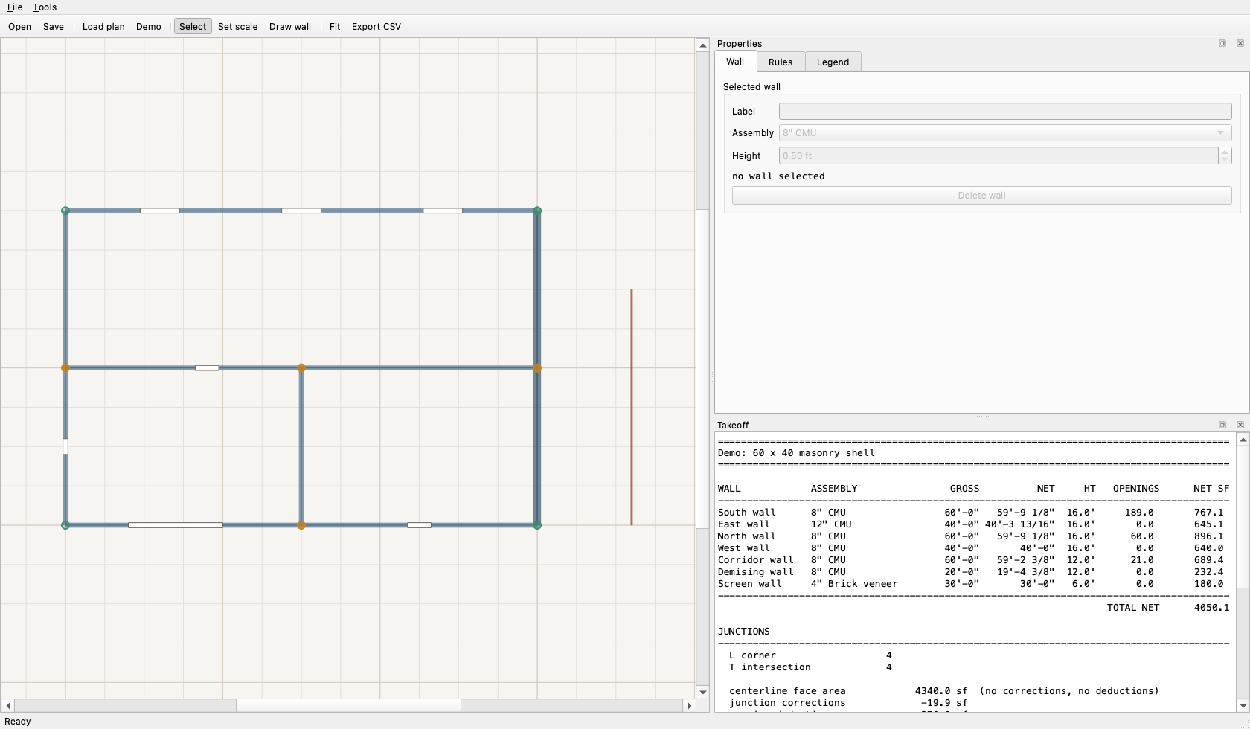
\includegraphics[width=\textwidth]{img/app.png}
\caption{The application with no plan underlay, so the grid shows. Walls are
stroked at true thickness, blue for block and red for the brick screen wall.
White rectangles are openings. The right-hand docks are the wall properties
and the live takeoff report.}
\end{figure}

\subsection{\texttt{theme.py} (54 lines)}

Colours and fonts in one place. A paper-coloured canvas rather than a dark
IDE, because estimators work from printed and scanned drawings. Junction dot
colours carry meaning: green for a corner that needed nothing, amber for one
that moved material, red for a crossing, purple for multi-way.

\subsection{\texttt{canvas.py} (437 lines)}

A \code{QGraphicsView} with a custom \code{drawBackground} for the plan
underlay and grid, and \code{drawForeground} for walls, openings and
junction dots.

Scene coordinates are plan-image pixels; the model stores feet;
\code{px\_per\_ft} is the only thing that converts, deliberately in one
place.

\textbf{Walls are stroked at their real thickness} with flat caps and mitre
joins, not drawn as hairlines. That is how masonry actually meets, and it is
why you can see the overlap at a junction.

\begin{keypoint}[A bug worth knowing about]
The obvious way to make plan $y$ point up is \code{view.scale(1, -1)}. That
also mirrors the background image, so every loaded plan renders upside down.
The fix is to negate $y$ at the single feet-to-scene conversion boundary
instead. There is a comment in \code{to\_scene} explaining it.
\end{keypoint}

\subsection{\texttt{panels.py} (215 lines)}

\code{WallPanel} edits the selected wall and shows its gross length, junction
adjustment, net length, area and unit count. \code{RulesPanel} exposes the
waste factor and the opening deduction threshold, so the estimating
assumptions are visible rather than buried. \code{ReportPanel} is the live
takeoff. \code{JunctionLegend} explains the dot colours.

\subsection{\texttt{app.py} (368 lines)}

\code{MainWindow}: toolbar, menus, docks, and the edit-to-report loop.

Every edit re-runs the entire takeoff. A 220-wall plan solves in about 7 ms,
so a dependency graph would be more code, more state, and a new class of bug
where the screen disagrees with the model.

\code{\_on\_junction\_clicked} is the feature worth demoing: click a dot and
the status bar says what that junction did and why, in the same words the
report uses.

\section{Top-level modules}

\subsection{\texttt{demo.py} (83 lines)}

A 60x40 masonry shell built to exercise every junction type: four L corners
(two of them mixed-assembly, because the east wall is 12" block), four T
intersections, two materials, and openings both over and under the deduction
threshold. Plus a freestanding brick screen wall, because masonry
contractors bid those and it puts a second material in the bill without
inventing a strange cavity detail.

\code{demo\_project\_on\_plan()} translates the same building onto the
rendered sample drawing so the overlay lines up without anyone tracing it by
hand. The offset is derived from the generator's constants, not measured by
eye, so the two stay in step.

\subsection{\texttt{cli.py} (100 lines)}

\code{report}, \code{export}, \code{save-demo}, \code{bench}, \code{ui}. The
CLI is not a side feature; it is the proof that Qt really is confined to
\code{ui/}.

\subsection{\texttt{bench.py} (190 lines)}

Two generators (\code{lattice}, where every wall spans the plan, and
\code{rooms}, short wall runs) and a timing harness that reports both stages
separately.

\begin{keypoint}[The benchmark records a mistake on purpose]
The pair scan looked like the bottleneck and was not. Profiling showed 3 ms
in intersection testing against 229 ms in clustering. Both implementations
are kept so the numbers can be shown, including the unflattering column
where the index eliminates zero pairs.
\end{keypoint}

\section{\texttt{tools/make\_demo\_plan.py} (158 lines)}

Generates \code{assets/demo\_plan.pdf} with pymupdf: walls as double lines
with gaps and jambs at the openings, dimension strings with ticks, suite
labels, a title block and a scale note. Drawn at 1/8" = 1'-0", which is 9
points per foot on letter landscape. A development tool, not part of the
installed package.

\begin{figure}[h]
\centering
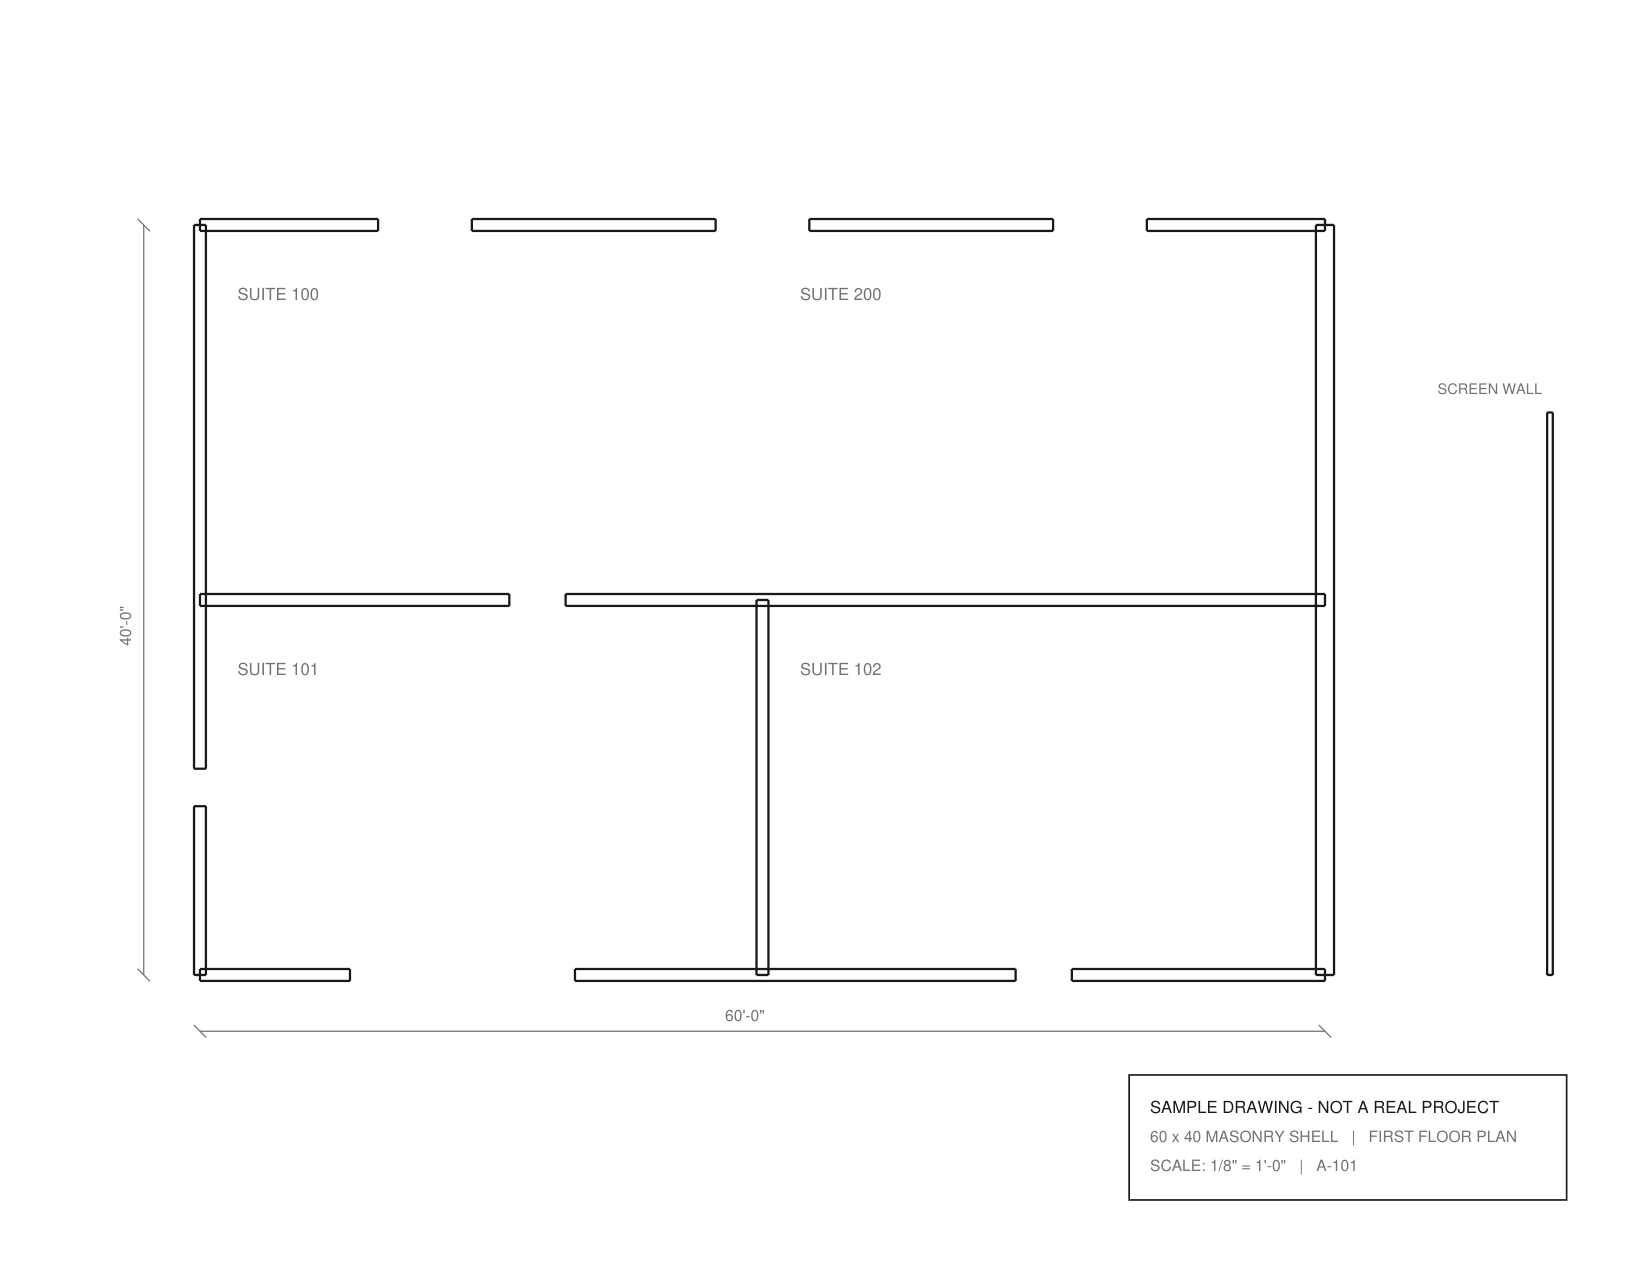
\includegraphics[width=0.92\textwidth]{img/demo_plan.png}
\caption{The generated sample drawing. Walls as double lines, gaps with
jambs where openings are, dimension strings, suite labels, and a title block
giving the scale. Labelled "SAMPLE DRAWING \textendash\ NOT A REAL PROJECT"
because it is synthetic.}
\end{figure}

\section{\texttt{tests/} \textendash\ 177 tests}

\begin{center}
\begin{tabular}{@{}lp{8.1cm}@{}}
\toprule
\textbf{File} & \textbf{What it covers} \\
\midrule
\code{oracle.py} & Not a test. The independent shapely oracle others use \\
\code{plans.py} & Synthetic plan generators shared by several suites \\
\code{conftest.py} & Sets \code{QT\_QPA\_PLATFORM=offscreen} before Qt imports \\
\code{test\_known\_answers.py} & 14 hand-computable cases, arithmetic in each docstring \\
\code{test\_oracle.py} & 46 tests comparing the solver to the polygon oracle \\
\code{test\_properties.py} & Translation, rotation, ordering, reversal, scaling invariance \\
\code{test\_takeoff.py} & Quantity arithmetic against textbook figures \\
\code{test\_units.py} & 30 parse and format cases \\
\code{test\_store.py} & Round trips, migrations, cascades, failed-save rollback \\
\code{test\_ui.py} & The window driven headlessly \\
\code{test\_layering.py} & Parses every module's AST; fails if Qt escapes \code{ui/} \\
\code{test\_end\_to\_end.py} & Renders the sample PDF, calibrates, checks the scale \\
\bottomrule
\end{tabular}
\end{center}

\subsection{The oracle, which is the point}

\code{tests/oracle.py} merges every wall centerline into connected linework
and lets shapely buffer it by half the thickness with mitred joins, then
measures the polygon's area.

\begin{keypoint}[Why this is strong evidence]
It shares no code and no reasoning with the solver. It does not know what a
T intersection is. They agree to one part in $10^9$ across closed shells, 25
randomly generated buildings, all four thicknesses, and $n \times n$
lattices of nothing but crossings. Shapely is a \emph{test-only} dependency
and \code{test\_layering.py} fails if it ever appears under \code{src/}.
\end{keypoint}

\section{\texttt{docs/} and \texttt{assets/}}

\begin{itemize}
  \item \code{DECISIONS.md} \textendash\ six architecture decision records:
    analytic corrections vs polygon booleans, shapely as a test-only oracle,
    SQLite over JSON, the centerline tracing convention, Qt confined to
    \code{ui/}, and recomputing on every edit.
  \item \code{CODE-TOUR.md} \textendash\ the Markdown source of this
    document, which is what GitHub renders.
  \item \code{assets/demo\_plan.pdf} \textendash\ the generated sample
    drawing, labelled synthetic in its title block.
\end{itemize}

\section{The images}

All three live in \code{docs/img/} and all three are generated, not
hand-made.

\code{demo\_plan.png} is page one of \code{assets/demo\_plan.pdf} rasterised
at 110 dpi. \code{app.png} is the application with no underlay.
\code{app\_plan.png} is the same building traced over the drawing, and it is
the more useful one, because the alignment is a visual proof that the scale
calibration maths is right.

Both screenshots are captured headlessly on Qt's offscreen platform, so they
regenerate on any machine including CI.

\begin{lstlisting}[language=none]
# the plan
python tools/make_demo_plan.py assets/demo_plan.pdf
python -c "import pymupdf; pymupdf.open('assets/demo_plan.pdf')[0] \
           .get_pixmap(dpi=110).save('docs/img/demo_plan.png')"

# the screenshots: see docs/CODE-TOUR.md for the full script
QT_QPA_PLATFORM=offscreen python scripts_snapshot.py
\end{lstlisting}

\section{\texttt{.github/workflows/ci.yml}}

Two jobs. \code{test} runs ruff and pytest on Python 3.11, 3.12 and 3.13,
with \code{fail-fast: false} so one version failing still reports the
others. It installs Qt's runtime libraries explicitly, because without them
Qt cannot load even its offscreen platform plugin and you get a confusing
plugin error rather than a test failure. \code{benchmark} runs the junction
benchmark so the numbers stay honest.

\section{One edit, traced end to end}

What happens when you drag a wall in the app:

\begin{enumerate}
  \item \code{canvas.py} handles the mouse event and converts scene pixels
    to feet through \code{to\_feet}.
  \item The wall's vertices change on the \code{Wall} dataclass.
  \item \code{app.py:refresh()} calls \code{takeoff.build(project)}.
  \item \code{takeoff.build} calls \code{junctions.solve}, which rebuilds the
    segment list, finds candidate pairs through the grid hash, intersects
    them, classifies each contact as END or BODY, clusters hits into nodes,
    and applies one correction per junction kind.
  \item \code{takeoff.build} turns net lengths into areas, subtracts
    openings over the threshold, and aggregates per assembly.
  \item \code{render.as\_text} formats it and \code{ReportPanel} displays it.
  \item \code{canvas.py} repaints with the new junction set.
\end{enumerate}

About 7 ms for a 220-wall plan, which is why step 3 re-runs everything
rather than trying to be clever.

\end{document}
